\documentclass[a4paper,
fontsize=11pt,
%headings=small,
oneside,
numbers=noperiodatend,
parskip=half-,
bibliography=totoc,
final
]{scrartcl}

\usepackage{synttree}
\usepackage{graphicx}
\setkeys{Gin}{width=.4\textwidth} %default pics size

\graphicspath{{./plots/}}
\usepackage[ngerman]{babel}
\usepackage[T1]{fontenc}
%\usepackage{amsmath}
\usepackage[utf8x]{inputenc}
\usepackage [hyphens]{url}
\usepackage{booktabs} 
\usepackage[left=2.4cm,right=2.4cm,top=2.3cm,bottom=2cm,includeheadfoot]{geometry}
\usepackage{eurosym}
\usepackage{multirow}
\usepackage[ngerman]{varioref}
\setcapindent{1em}
\renewcommand{\labelitemi}{--}
\usepackage{paralist}
\usepackage{pdfpages}
\usepackage{lscape}
\usepackage{float}
\usepackage{acronym}
\usepackage{eurosym}
\usepackage[babel]{csquotes}
\usepackage{longtable,lscape}
\usepackage{mathpazo}
\usepackage[normalem]{ulem} %emphasize weiterhin kursiv
\usepackage[flushmargin,ragged]{footmisc} % left align footnote

\usepackage{listings}

\urlstyle{same}  % don't use monospace font for urls

\usepackage[fleqn]{amsmath}

%adjust fontsize for part

\usepackage{sectsty}
\partfont{\large}

%Das BibTeX-Zeichen mit \BibTeX setzen:
\def\symbol#1{\char #1\relax}
\def\bsl{{\tt\symbol{'134}}}
\def\BibTeX{{\rm B\kern-.05em{\sc i\kern-.025em b}\kern-.08em
    T\kern-.1667em\lower.7ex\hbox{E}\kern-.125emX}}

\usepackage{fancyhdr}
\fancyhf{}
\pagestyle{fancyplain}
\fancyhead[R]{\thepage}

%meta

%meta

\fancyhead[L]{Redaktion LIBREAS \\ %author
LIBREAS. Library Ideas, 30 (2016). % journal, issue, volume.
\href{http://nbn-resolving.de/
}{}} % urn
\fancyhead[R]{\thepage} %page number
\fancyfoot[L] {\textit{Creative Commons BY 3.0}} %licence
\fancyfoot[R] {\textit{ISSN: 1860-7950}}

\title{\LARGE{Editorial \#30: Post-Digital Humanities}} %title %title
\author{Redaktion LIBREAS} %author

\setcounter{page}{1}

\usepackage[colorlinks, linkcolor=black,citecolor=black, urlcolor=blue,
breaklinks= true]{hyperref}

\date{}
\begin{document}

\maketitle
\thispagestyle{fancyplain} 

%abstracts

%body
\section*{Motivation für die
Ausgabe}\label{motivation-fuxfcr-die-ausgabe}

Warum Post-Digital-Humanities? Eine Antwort auf diese Frage haben wir
Call for Papers dieser Ausgabe zu formulieren versucht. (LIBREAS.
Redaktion, 2016) Im seitdem vergangenen halben Jahr ist uns nichts
begegnet, was uns zu einem grundsätzlichen Abweichen von dieser Position
motivieren konnte.

Wir gingen davon aus, dass sich \enquote{Post-Digital-Humanities} als
eine Art Gegenlabel sowohl zu den traditionellen Geisteswissenschaften
als auch zu den Digital Humanities anbieten. Das Potential dieses
Ansatzes, so schrieben wir, \enquote{liegt in der Öffnung eines
dekonstruktiven und damit das Selbstverständnis hinterfragenden und
zugleich voran bringenden Ansatzes. Denn ein allen Geisteswissenschaften
gemeinsames Merkmal ist der Diskurs, der auch das Hinterfragen der
eigenen Methoden beinhaltet.} (ebd.)

Da \enquote{post-digital} als Begriff, wie wir unten noch einmal
benennen, im Prinzip seine eigene Überflüssigkeit beinhaltet, ist sein
einziger Zweck tatsächlich der einer Bewusstmachung. So wie die Idee der
Postmoderne jegliche Bildung von Schulen und Ideologien notwendig
unterlief, ist die Attributierung von \enquote{post-digital} eine
diskursiver Hebel, um das vermeintlich Selbstverständliche zu
konfrontieren. Und zwar einerseits mit einer Vielzahl von näheren und
entfernteren Entwicklungen und andererseits immer auch mit sich selbst.

Zu den näheren Einflüssen lässt sich aus dem Call festhalten:

\begin{quote}
\enquote{Postdigitale geisteswissenschaftliche Arbeit ist {[}\ldots{}{]}
eine wissenschaftliche Praxis, die sich unter dem Einfluss und auch mit
den Mitteln digitaler Technologien, Netzwerke und Kultureffekte
vollzieht. Das Spektrum reicht von n-gram-Analysen bis zu Altmetrics,
beinhaltet also in etwa all das, was in der vordigitalen Wissenschaft
weder möglich noch ahnbar war. Damit wird sie sinnvoll über das engere
Feld der Digital-Humanities-Anwendungen erweiterbar, das de facto vor
allem im Bereich der Analyse großer Datenmengen, beispielsweise der
Korpuslinguistik oder auch der digitalen Mustererkennung für die
Kunstgeschichte ihre überzeugendsten Konkretisierungen erfährt.} (ebd.)
\end{quote}

Die weiteren Einflüsse betreffen unter anderem die Kanäle, über die
geisteswissenschaftliche Erkenntnisse kommuniziert werden. Also zu
großen Teilen die Bibliotheken, die traditionell Publikationen als
formale Diskursträger sammeln, erschließen und verfügbar halten.
Post-Digital-Humanities sind daher zwangsläufig auch ein Thema der
Bibliotheks- und Informationswissenschaft. Und zwar auch hinsichtlich
ihrer Abgrenzung, wie Sandra Balck in ihrem Beitrag zu dieser Ausgabe
heraus arbeitet.) Wenn es der Disziplin gelingt, mit ihrem
Überblicksverständnis zu den Entwicklungen des Digitalen relevant
Expertise in die Geisteswissenschaften zu vermitteln, dann erfüllt sie
exakt ihre Aufgabe. Und sie wäre in der Lage, einen stabilen Gegenpol zu
dem stetigen \enquote{prognostischen Unbehagen} zu entwickeln, dass
Bibliotheken regelmäßig gegenüber medialen Veränderungsprozessen hegen.
(Ausführlich schreibt dazu Andreas Hartsch in seinem Beitrag.)

\begin{figure}
\centering
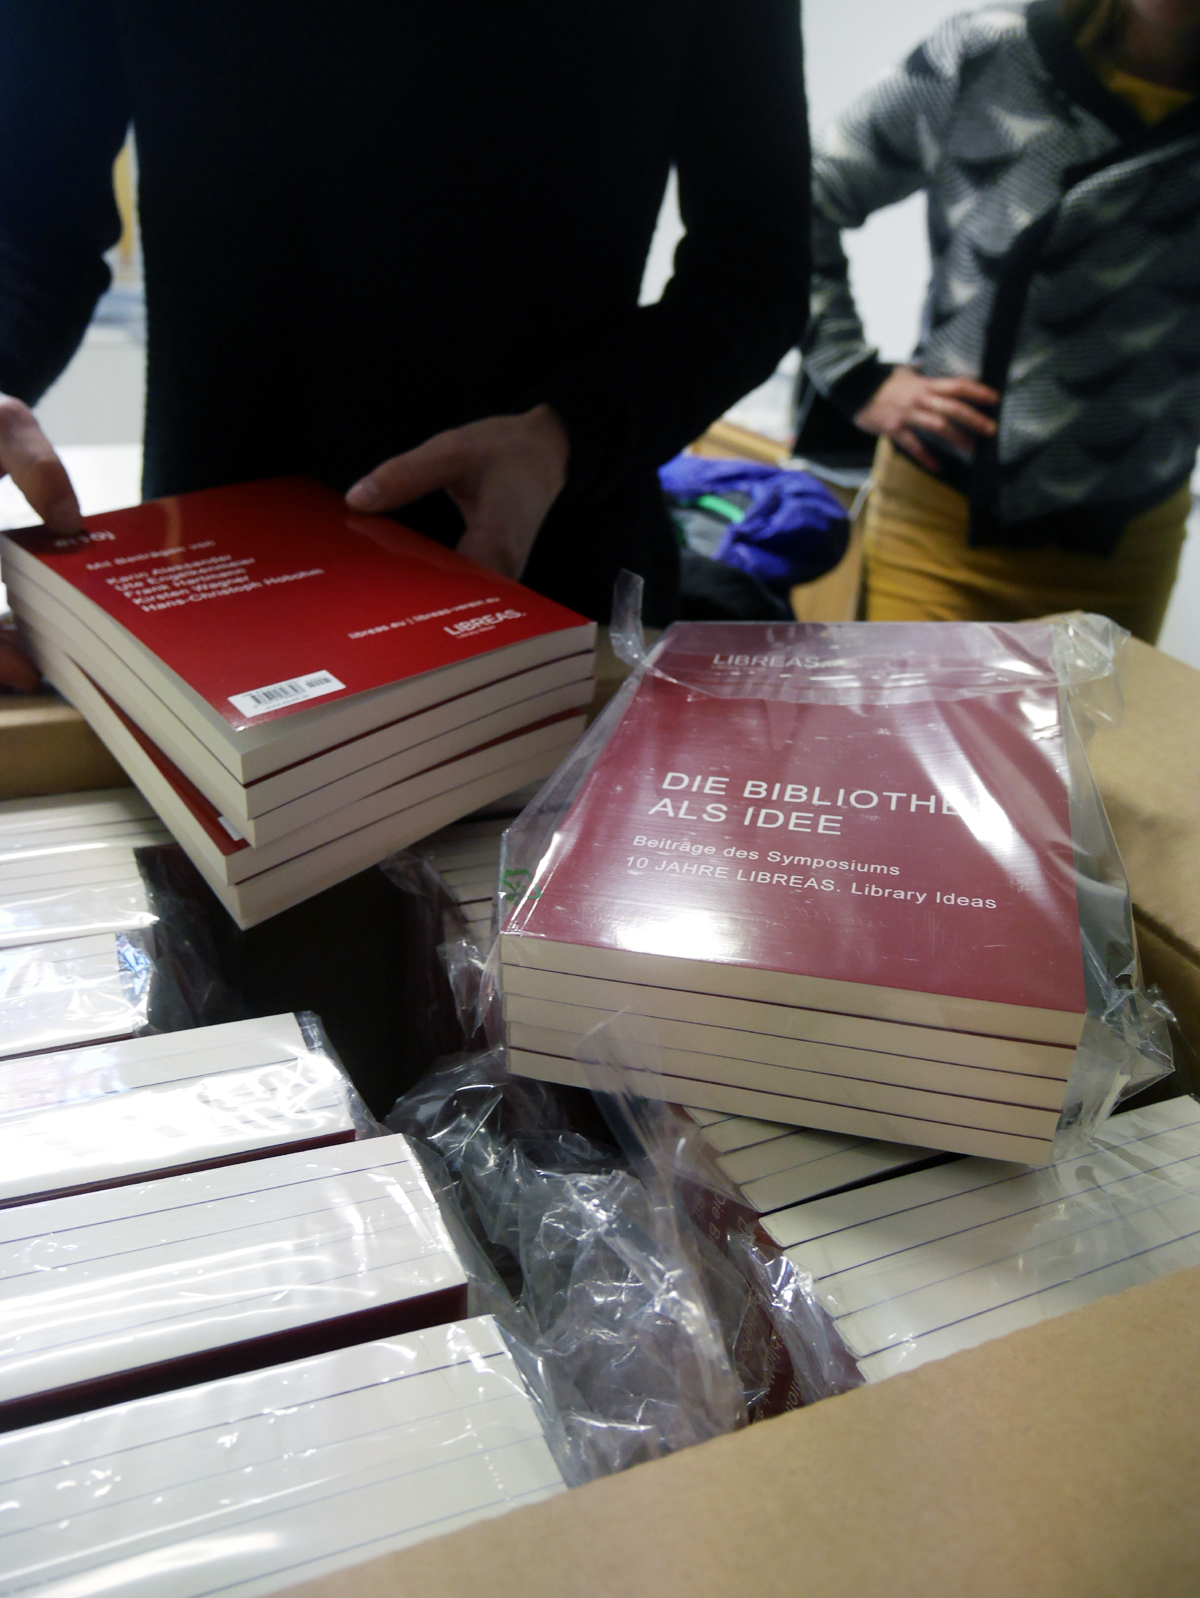
\includegraphics{redaktionssitzung.jpg}
\caption{Redaktionsorte: Akzession der Jubiläumsausgabe (Berlin, 16.
November 2016)}
\end{figure}

Wenigstens aus unserer Sicht ist das zeitgemäße Forschungsfeld der
Bibliotheks- und Informationswissenschaft weniger, wie Bibliotheken
digitale Systeme für die Optimierung ihrer traditionellen Aufgaben
nutzen, sondern die Frage, wie wissenschaftliche Kommunikation und
wissenschaftliches Publizieren unter dem Einfluss digitaler Technologien
zu verstehen und zu gestalten sind. Die Bibliotheks- und
Informationswissenschaft kann zudem als eine Art Meta-Wissenschaft ihre
Erfahrung in puncto Digitalisierung von Kulturobjekten als auch ihre
Expertise in der Elektronisierung von wissenschaftlichen Arbeitsabläufen
einbringen.

\section*{Postinternet / postdigitale Wissenschaften - eine
Begriffsbestimmung}\label{postinternet-postdigitale-wissenschaften---eine-begriffsbestimmung}

Die Idee, Begriff und Bezeichnung des Post-Digitalen kommen zunächst aus
der Kunst beziehungsweise eigentlich aus der elektronischen Musik, woran
Florian Cramer unlängst erinnerte. (Cramer, 2016) Abstrakter und im
gesellschaftlichen Rahmen bedeutet es, dass das Digitale
quasi-alternativlos ist. Selbst wenn wir Print lesen, stehen dahinter
digitale Technologien und eben keine Schriftsetzer und Druckstöcke mehr.
Zugleich zeigt sich, dass das \enquote{Digitale} doch keine Revolution
ist. Oder keine mehr. Das Digitale ist die Fortsetzung der Trivialitäten
des Alltags mit anderen Mitteln. Und, wie man oft festzustellen
vermeint, ihre Entgrenzung. Florian Cramer zielt zurück auf Alessandro
Ludovico und stellt mit diesem fest, dass das mit Vehemenz postulierte
anstehende Ende des Gedruckten fast notwendig ausbleiben musste.

\begin{quote}
\enquote{Print und Elektronik {[}stehen{]} daher nicht im Gegensatz von
\enquote{altem} und \enquote{neuen} Medium, sondern erfordern neue,
analog-digitale Kombinationen. Wie die postdigitalen Musiker im Jahr
2000, argumentierte Ludovico im Jahr 2012, dass Digitaltechnologie nicht
per se Fortschritt und Zukunft bedeute.} (ebd.)
\end{quote}

Historisches Verständnis lehrt, dass sich seit je lineare und absolute
Aussagen darüber, wie etwas sein wird, am Ende sehr häufig als
überschaubare Egoprojekte erweisen, die einen bestimmten individuellen
Wirkungswunsch, nicht aber die grundsätzliche Komplexität von in
Wechselwirkungen dahinfließender Systeme als zentrale Größe definieren.
Insofern ist Vorsicht bei allzu scharfen Verkündungen und
Alternativlosigkeitsbehauptungen geboten. Denn wie eigentlich jede/r
weiß, ist es bei Technologie- und Gesellschaftsentwicklung zweckmäßiger,
statt auf langfristige Prophezeiungen auf eine Kombination aus stabilen
Grundwerten und iterative Analysen der jeweiligen Gegenwart unter
Berücksichtigung bestimmter und abschätzbarer Wahrscheinlichkeiten zu
setzen. Dann bleibt vielleicht manche \enquote{Disruption} aus. Dafür
sind die Ergebnisse aber belastbarer und inklusiver. Zudem verpasst man
die wirklichen Bruchstellen meist ohnehin sowieso trotz aller
Hype-Zyklen. Das vermeintlich Revolutionäre fällt dagegen sehr
regelmäßig in oft nicht nur angenehme bekannte Muster zurück.

Die Aufgabe von Kritik, wie auch wir von LIBREAS sie verstehen, ist,
beständig daran zu erinnern und auch daran, dass eine ideologische
Hingabe gleich welcher Art, also egal ob an kommunistische Manifeste,
den Apple-Chic , ein großes Amerika oder die Open-Access-Bewegung früher
oder später die Ausfahrt zu einer handhaberen Realität verpassen müssen.
Selten wurde das in einer Ballung deutlicher als in diesem eigenartigen
Jahr 2016.

\section*{Post-Internet=Die Allgegenwart der
Commons?}\label{post-internetdie-allgegenwart-der-commons}

Das spielt deutlich mit einem weiteren von Florian Cramer thematisierten
Aspekt zu Post-Internet- und Post-Medienkulturen zusammen:

\begin{quote}
\enquote{Die{[}se{]} Begriffe drücken ein Bedürfnis aus, Kunst unter
{[}\ldots{}{]} veränderten technisch-geopolitisch-bildkulturerellen
Bedingungen zu beschreiben, die spätestens seit Edward Snowden nicht
mehr zu leugnen sind. Im Zeitalter elektronischer Totalüberwachung ist
jede und jeder, ob gewollt oder nicht, Performancekünstler und
Netzpublizist -- und sei es nur durch Überweisen der Miete.} (Cramer,
2016, S.66)
\end{quote}

Entsprechend klar ist, dass eine Schranke auch zwischen Kunst und
Wissenschaft an dieser Stelle hinfällig ist. Das Post-Digitale ist nicht
mehr Kunst oder Wissenschaft oder Humanities. Es ist ebenfalls total.
Als Einsicht ist das wichtig. Aber was können wir damit machen? Bedeutet
im alltäglichen Prozessieren von Wirklichkeit und Deutung
\emph{postdigital} dann nichts anderes, als einfach einen Zustand
ubiquitärer Vernetzung und Interaktion mittels entsprechender
Technologien? Also, dass das Digitale so selbstverständlich ist, dass
jede Hervorhebung überflüssig wirkt? David Berry notierte 2014 als
Gegenwartsbeschreibung:

\begin{quote}
\enquote{Indeed, just as the ideas of \enquote{online} or \enquote{being
online} have become anachronistic as a result of our always-on
smartphones and tablets and widespread wireless networking technologies,
so too the term \enquote{digital} perhaps assumes a world of the past.}
(Berry, 2014)
\end{quote}

Für uns in diesem Rahmen Agierende bedeutet es: \emph{die digitale
Revolution ist vorbei}. Willkommen zu den Mühen des Alltags. Auch das
ist heilsam, nicht zuletzt für die sich selbst erklärenden Digital
Humanists, die verstehen müssen, dass sie dann, wenn sie ihre
Wissenschaftspraxis auf ein Revolutionsversprechen zu gründen versuchen,
etwa 15 Jahre zu spät kommen. Post-Digital-Humanities sind kein Umsturz
der Geisteswissenschaften, sondern ein doppeltes
Normalisierungsgeschehen. Ihre Aufgabe ist es, das Digitale -- also
Technologien, Interaktionsformen, Erkenntnismöglichkeiten -- in die
Geisteswissenschaften zu bringen und zugleich die Geisteswissenschaften
-- Methodologien, Erkenntniskompetenzen -- auf das Digitale zu spiegeln.
Post-Digital-Humanities sind kein erfürchtiges Bestaunen von
Visualisierungen mehr, sondern eine kritische Anfrage zur
Digitalisierung: Wo und wozu?

Dies gilt auch für die Frage, in welcher Form wir wollen, dass in
digitalen Strukturen entwickelte Prinzipien auch auf Nicht-digitale
Zusammenhänge zurückwirken. Besonders deutlich wird dies im
Wiederaufkommen von Allmende-Ideen, oft unter dem Label der Commons, die
eine erstklassige Projektionsfläche für die Erben der linken
Ideengeschichte darstellen. Florian Cramer beschreibt aktuell die
Perspektive der Filmemacherin Hito Steyerl:

\begin{quote}
\enquote{Tatsächlich geht es Steyerl um die veränderte Zirkulation von
Bildern und die Ausweitung von \enquote{Open Access}-Prinzipien von
digitalen Dateien auf \enquote{Wasser, Energie und Dom
Pérignon-Champagner}} (Cramer, 2016)
\end{quote}

Das freie Zirkulieren ist das Grundprinzip und führte mit
neokommunistischen Utopien wie der von Hito Steyer in ein ganz anderes
\enquote{Internet der Dinge}:

\begin{quote}
\enquote{If copyright can be dodged and called into question, why can't
private property? If one can share a restaurant dish JPEG on Facebook,
why not the real meal? Why not apply fair use to space, parks, and
swimming pools? Why only claim open access to JSTOR and not MIT -- or
any school, hospital, or university for that matter? Why shouldn't data
clouds discharge as storming supermarkets? Why not open-source water,
energy, and Dom Pérignon champagne?} (Steyerl, 2013)

\enquote{If circulationism is to mean anything, it has to move into the
world of offline distribution, of 3D dissemination of resources, of
music, land, and inspiration. Why not slowly withdraw from an undead
internet to build a few others next to it?} (Steyerl, 2013)
\end{quote}

Wir müssen an dieser Stelle die praktischen Hürden dieses Gedankenspiels
außen vorlassen. Es geht einzig darum, zu registrieren, dass das
Post-Internet einen politischeren Kern enthalten kann, als man zunächst
unter anderem auch nach der Inaugenscheinnahme entsprechend gelabelter
Kunstschauen vermuten möchte.

\section*{Die Informationsethik an doppelter
Front?}\label{die-informationsethik-an-doppelter-front}

Aus der Sicht der Bibliothekswissenschaft steht die Informationsethik
wieder ganz vorn in der Verantwortungskette. Bekanntlich schuftet sie
sehr engagiert zumindest auf dem Open-Access-Feld und zwar an doppelter
Front: Den wissenschaftlichen Großverlagen, die es vermochten, sich in
aller pop- und postmodernen Raffinesse ein progressives Thema
anzueignen, um auf dem Grundnarrativ Geschäftsmodelle aufzupropfen, die
unter dem Strich wieder Bilanzen erscheinen lassen, die in den 1990er
Jahren mit der Bezeichnung Zeitschriftenkrise erst zur Entstehung der
Open-Access-Bewegung führten. (Und die mit Schattenbibliotheken dort
eine Art Grassroots-\emph{Remedium} fand, wo Bedarf und Bequemlichkeit
nicht mit Angebot und Nutzungsbedingungen für wissenschaftliche
Publikationen übereinstimmen, wie Eric Steinhauer in seinem Beitrag über
Sci-Hub ausführt.)

Die andere Front sind Buchverlage und versprengte Akteure aus den
Geisteswissenschaften und dem Bibliothekswesen, die genau diese Gefahr
attackieren, jedoch nicht die Gefahrenquelle, sondern vielmehr alle
anderen, die in der Mitte unterwegs sind und sich fragen, wie
(post)digitales Publizieren eigentlich sinnvoll aussehen kann.(Kaden,
2016a)

Auf der Ebene des entsprechenden Diskurses zeigt sich daher, dass ein
sanfteres Denken in Richtung Wissensallmende -- deren Vorstufe die Idee
der Öffentlichen beziehungsweise öffentlich nutzbaren Bibliothek war --
von zwei Seiten angegriffen wird, deren gemeinsames Merkmal das
expansive Verankern bestimmter Geschäftsmodelle ist. Während die großen
Wissenschaftsverlage schlicht auf den Rücken des Open-Access-Zeitgeistes
aufsatteln, arbeiten sich die Verleger des guten Fach- und Lehrbuches an
einer vermeintlichen Gefährdung von Grundrechten ab, die für sie dann
vorliegt, wenn Wissenschaftlerinnen und Wissenschaftler andere Kanäle
zur Kommunikation ihres Wissens zur Verfügung haben, als die, die diese
Verlage kontrollieren. (Siehe dazu auch den Beitrag von Thomas Ernst in
dieser Ausgabe.)

Dass die Sprecher (offenbar nur Sprecher, was vielleicht auch etwas über
diese Debatte sagt) der letztgenannten Position in erstaunlicher
Beharrlichkeit die Binarität von Digital zu Analog ausspielen, ist nur
scheinbar ein Anachronismus. Bei genauerer Betrachtung folgen sie,
bewusst oder unbewusst, höchst gegenwärtigen Diskursstrategien, die
aktuell -- ein weiteres \enquote{post} -- also postfaktisch beschrieben
werden. In Deutungsräumen die eben nicht ein-deutig bestimmbar sind,
sondern vielmehr unendliche Vernetzungen und Verästelungen zulassen,
trumpft die einfache Behauptung jede Unsicherheit. Die Strategie ist,
griffige Marker zu kommunizieren, mit denen sich die jeweiligen
Zielgruppen assoziieren können. Ein Beispiel ist die Behauptung, Open
Access gefährde die Wissenschaftsfreiheit und führe zwangsläufig in
einen Publikationszwang. Eine weitere Strategie ist, nur Prämissen zu
konstruieren, die zwar keine realite und logische Basis haben, jedoch
einfache Zielscheiben darstellen, anhand derer das verunsicherte
Publikum überzeugt werden soll. Was in gesellschaftspolitischen
Zusammenhängen leider gefährlich gut funktioniert, läuft in
wissenschaftlichen Kontexten glücklicherweise meist ins Leere, da diese
Zielgruppen im Ergebnis Logik und Beleg stärker als Alarmismus und
Behauptung gewichten.

\section*{Nach dem Binären}\label{nach-dem-binuxe4ren}

Eine der faszinierendsten Eigenschaften des Post-Digitalen ist, mit
welcher Zielstrebigkeit der Einfluss digitaler Kommunikationspraxen dazu
führt, Binaritäten aufzulösen. Transdiskursive Kompetenz ist die
Fertigkeit der Stunde und übrigens auch der Bibliotheken, die sich mehr
als Diskurs- denn als Bestandsvermittler verstehen müssen. Wie könnte
man Katja Kwastek widersprechen, wenn sie schreibt, \enquote{dass das
Digitale auch andere Diskursformen mit sich bringt}? (Kwastek, 2016, S.
80) Genaugenommen ist das ein Gemeinplatz und auch nicht ganz stimmig,
denn das Digitale manipuliert bestehende Praxen des Diskurses. Die
Herausforderung besteht nicht zuletzt für digitale Wissenschaft darin,
die entsprechende Prozesse und Auswirkungen zu verstehen und in der
Folge zu entscheiden, ob man diesen folgen oder sie gestalten möchte.
Will man sie gestalten, ist eine bedeutete Facette der
Post-Digital-Humanities die Auseinandersetzung mit der Frage, wie
Wissenschaft digital kommuniziert. Denn was Katja Kwastek bei ihrer
Reflexion über eine \enquote{Postdigitale Kunstwissenschaft?}
beschreibt, ist eine zwar sehr zutreffende doch eher eine simple
Grunddiagnose:

\enquote{Heterogene Forschungs- und Publikationsplattformen und schnelle
Online-Diskussionen lassen oft zunächst einmal jeden Autor und Beitrag
zu. Erfolg hat, wem es gelingt, genug Aufmerksamkeit auf sich zu ziehen.
Reputationssysteme ersetzen die Kanonwächter. Sicher ist ein bloßes
\enquote{Liken} oder \enquote{Retweeten} noch kein qualitativ
differenzierter Diskurs, aber hier obliegt es letztlich den Nutzern
selbst, entsprechend intelligente Systeme zu entwickeln.} (Kwastek,
2016, S.80)

In eine ähnliche Richtung weist die Erläuterung der Siggenthese \#10:

\begin{quote}
\enquote{Die Zukunft wird durch die Beteiligten gestaltet, somit
beeinflussen wir die Gültigkeit unserer eigenen Prognosen. Da der
Gestaltungsprozess grundsätzlich in einem Interessenwiderspruch
stattfindet und der Diskurs dazu über weite Strecken von
durchsetzungsgetriebener Rhetorik geprägt wird, ist es erforderlich, die
eigenen Ziele und Interessen eindeutig und verständlich benennen zu
können.} (vgl. Kaden, 2016b)
\end{quote}

Es gilt zu bestimmen, welche Art von Geisteswissenschaften die
Post-Digital-Humanities sein wollen und welche Form von Diskurs sie als
zulässig definieren möchte. Und es gilt gleichermaßen, welche Rolle
Bibliotheken und andere Akteure der Organisation wissenschaftlicher
Diskurs übernehmen können und wollen. Die vorliegende LIBREAS-Ausgabe
wird dafür naturgemäß nur Impulse vom Rand geben können.

Ihre / Eure Redaktion LIBREAS. Library Ideas

(Berlin, Chur, Dresden, Hannover, München)

\section*{Quellen}\label{quellen}

David Berry: Post-Digital Humanities: Computation and Cultural Critique
in the Arts and Humanities. In: Educause Review, 19.05.2014,
\url{http://er.educause.edu/articles/2014/5/postdigital-humanities-computation-and-cultural-critique-in-the-arts-and-humanities}.

Florian Cramer: Nach dem Koitus oder nach dem Tod? Zur
Begriffsverwirrung von \enquote{Postdigital}, \enquote{Post-Internet}
und \enquote{Post-Media}. In: Kunstforum International, Bd. 242,
Sept.-Okt.2016. S. 54-67.

Ben Kaden (a): Die Entdeckung des „Faselns``. Der Stroemfeld-Verlag
sieht sich über dem Diskurs.In: LIBREAS. Weblog, 07.11.2016,
\url{https://libreas.wordpress.com/2016/11/07/stroemfeld/}.

Ben Kaden (b): Wissenschaftskommunikation auf Gut Siggen. Und zehn
Thesen als Ergebnis. In: LIBREAS. Weblog, 24.10.2016
\url{https://libreas.wordpress.com/2016/10/24/siggener-thesen-wissenschaftskommunikation/}.

Katja Kwastek: Wir sind nie digital gewesen. Postdigitale Kunst als
Kritik binären Denkens. In: Kunstforum International, Bd. 242,
Sept.-Okt.2016. S.68-81

LIBREAS.Redaktion: Post-Digital Humanities aus bibliotheks- und
informationswissenschaftlicher Sicht. In: LIBREAS. Weblog, 04.05.2016
\url{https://libreas.wordpress.com/2016/05/04/libreas-cfp-digital-humanities/}.

Hito Steyerl: Too Much World: Is the Internet Dead? In: e-flux Journal
\#49 - November 2013
\url{http://www.e-flux.com/journal/49/60004/too-much-world-is-the-internet-dead/}

%autor

\end{document}
